\documentclass[a4paper,12pt]{article}

%\usepackage{fontspec}
%\setmainfont{Times New Roman}
\usepackage[scaled=0.92]{helvet}
\usepackage{bbm}
\usepackage{amsfonts}
\usepackage{amsthm}
\usepackage{array}
\usepackage{tabu}
\usepackage{tabularx}
\usepackage[pdftex]{xcolor, graphicx}
\usepackage[utf8]{inputenc}
\usepackage[a4paper, total={6in, 9in}]{geometry}
\usepackage{enumerate}
\usepackage{setspace}
\usepackage{hyperref}
\usepackage{float}
\usepackage{natbib}
\usepackage{amsmath}
\usepackage{ragged2e}
\usepackage{rotating}
\usepackage{chngpage}
\usepackage{bibentry}
\usepackage{commath}
\usepackage{pdflscape}
\usepackage{booktabs}
\usepackage{subcaption}
\usepackage{tikz}
\doublespacing
\hypersetup{colorlinks=true, citecolor=black, urlcolor=blue, linkcolor=black}
\newcolumntype{C}[1]{>{\Centering\arraybackslash}p{#1}}
\geometry{left = 1in, right= 1 in, top= 1 in, bottom=1in}

\setlength\parindent{0pt}

%\date{August, 2019}
\author{Uzoma Iloanugo}
\title{Predicting the Severity of Car Accidents in Seattle}


\begin{document}
\maketitle

\section{Introduction}
The World Health Organisation (WHO) reports that about 20 to 50 million people suffer from non-fatal injuries from vehicle accidents globally every year. Some of the risk factors the WHO considers are speeding, driving under the influence of alcohol or other psychoactive substances, improper use of road safety equipment (helmet, seat belts etc.), distracting the driver, unsafe road infrastructure and so on. Also, the Center for Disease Control shows that every year in the United States, about 3 million people are involved in accidents that cause serious injury. In 2017, the cost to the US economy was huge at about \$75billion in medical care cost and lost productivity from vehicle accidents alone. The Seattle Department of Transportation’s annual traffic report show that there were 10,959 vehicle-related accidents reported by the police in 2017. The impact of vehicle accident on the economy and citizen's lives and property make it of interest to stakeholders and the government.

\subsection{Business Problem}
A comprehensive study that measures the risk factors and estimates how they predict the severity of road accidents will be of use to all parties involved. These include private citizens who bear the pain of the accidents; the cooperation and State government that bear the loss in productivity as a result of road accidents; and insurance companies that provide cover for road users. The objective of this project is to fill in the gap. Using data from road accidents in Seattle, we predict the severity of road accidents by considering some of the risk factors stated by the WHO and other factors provided by the police data on road accidents. The Washington State Department of Transport (WSDOT) reported that the common causes of accident specific to Seattle are speeding, intoxication, following cars too closely, defective equipment, poor vehicle maintenance and failure to yield right of way. The dataset we use to create a predictive model should measure these factors to a good extent to enable the algorithm learn and predict car accidents in out-of-sample data.\\

The remaining section of the project will introduce and explore the data, discuss the machine learning models implemented in the analysis, conduct test on the accuracy of models and recommend the best prediction model. Lastly, I provide some policy recommendations based on findings and conclude.

\section{Data}
The data used in the study is from the Seattle Department of Transport (SDOT). The dataset collects information on the event of vehicle accidents in Seattle. The information includes the location and other attributes related to the event provided by the Seattle Police Department (SPD). Some attributes that will be considered important for the analysis in the dataset includes – the severity of the accident, location, the number of people involved, number of vehicles, the junction types, under the influence, weather, road condition, light condition, and if the driver was speeding. Other attributes will be considered and the analysis will involve selecting appropriate attributes that best predict the target – the severity of the accident. The machine learning model will predict accident severity and distinguish between a vehicle accident leading to damage of property versus causing serious injuries.

\newpage
\section{Methodology}
In this section, I will explore the SDOT data and examine how some important features determine the severity of accidents. I will also discuss all the variable that were used as-is and the various types of transformation that was done on the dataset. Finally, I will describe the transformed SDOT dataset that was fed into the machine learning models.

\subsection{Exploratory Data Analysis}
In the exploration, I will discuss some of the pertinent features suggested by the World Health Organisation (WHO) and understand how they interact to determine accident severity. It is important to understand that the variable of interest is whether the accident resulted in the destruction of property or injury of a person. We should expect that the factors that determine these closely related outcomes will involve interaction between features. It is also worth noting that most of the features are categorical, therefore, the most appropriate way to have a first view of the data is using bar charts.\\

First, I plot the distribution of accidents in the dataset by weather condition. Figure \ref{fig1} shows that surprisingly, majority of the accidents in the dataset happened when the weather was clear. In trying to understand why this is the case, I consider how light condition and driving under the influence affect accidents severity when the weather is clear. Figure \ref{fig2} is a plot that decomposes the accident severity when the weather is clear by the light conditions and driving under the influence of psychoactive substances. What we note is that the when driver's were under the influence, the highest number occurred when the road was dark. Figure \ref{fig3} interacts speeding in varying light conditions under a clear weather. We see similar results that most accidents occured when driver's were speeding in dark roads. These results suggests poor lighting is a relevant determinant of accident. However, it does not clearly distinguish when accidents cause damage to property versus when it causes injuries. \\


\begin{figure}[H]
	\centering
	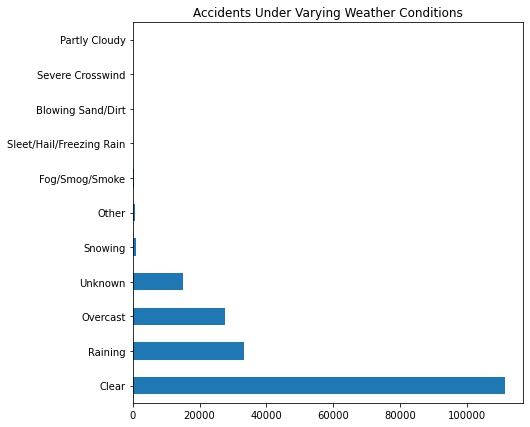
\includegraphics[width=0.8\textwidth]{weather.jpg}
	\caption{Weather conditions and accidents in Seattle.}
	\label{fig1}
\end{figure}


\begin{figure}[H]
	\centering
	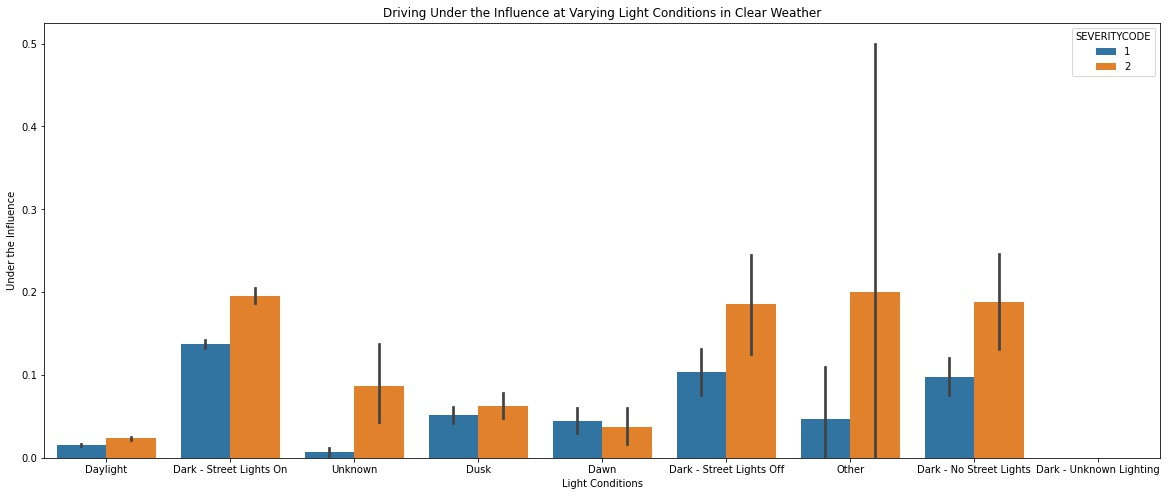
\includegraphics[width=1.0\textwidth]{li_un_wet.jpg}
	\caption{Accident severity by light condition and driving under the influence when the weather is clear. }
	\label{fig2}
\end{figure}

\begin{figure}[H]
	\centering
	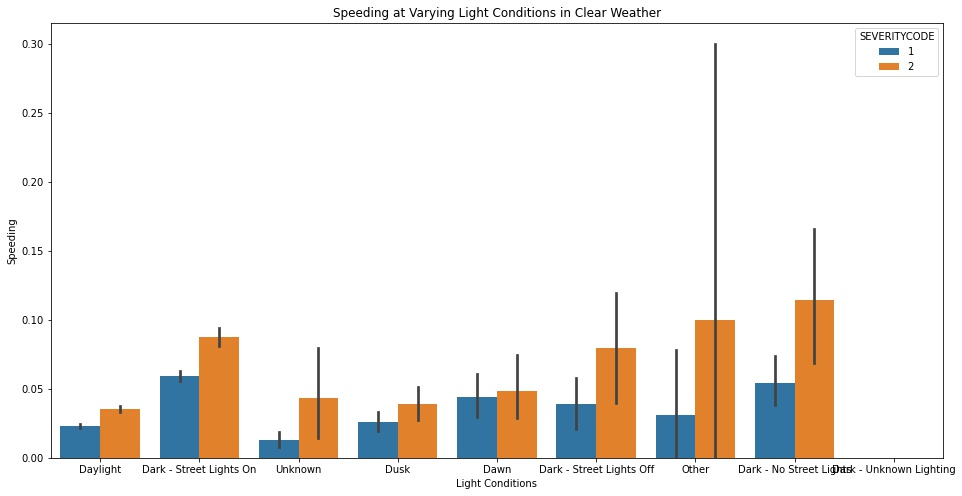
\includegraphics[width=1.0\textwidth]{li_sp_wet.jpg}
	\caption{Accident severity by light condition and speeding when the weather is clear.}
	\label{fig3}
\end{figure}

Next, I show how speeding under the influence of drugs contributes to accident severity in Seattle. Importantly, I check if speeding under the influence will clearly distinguish accidents that cause damage to property from accidents that cause injury. The bar chart in figure \ref{fig4} shows that majority of the incidents occurred when drivers were speeding under the influence of psychoactive drugs. Interestingly, we see that the category on the right of the plot shows a substantial difference between damage to property and injury related accidents.\\

We can see that speeding under the influence of psychoactive substances determine accidents severity in the dataset. Also, majority of the accidents occurred in dark roads. It is important to understand how poor light condition determine accident severity when the driver is speeding under the influence of psychoactive substances. Figure \ref{fig5} shows a bar plot of how light condition impact the severity of accidents when drivers speed under the influence of psychoactive substances. We note that most of the accidents occur in the dark where no street lights are available (The plot on the second facet). We also see that speeding under the influence when there is no street light strongly separates the accidents that cause damage to property and when they cause injury. So when a driver speeds under the influence of psychoactive substances in a dark street with no street light, accidents will more likely cause injury than accidents that destroy property. In general, what we understand so far is that to properly predict severity of accidents in Seattle, we need to interact the features in the dataset to clearly distinguish between the two types of accident in the target. \\

\begin{figure}[H]
	\centering
	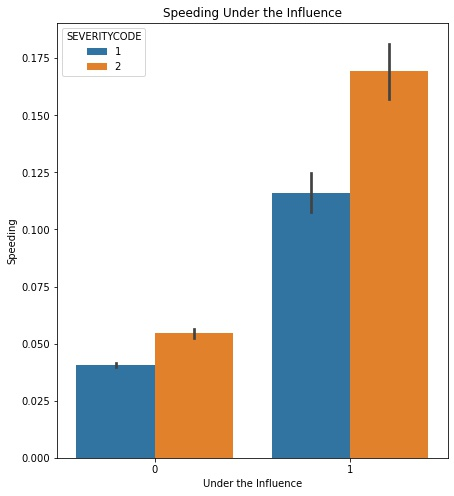
\includegraphics[width=0.6\textwidth]{un_sp_sev.jpg}
	\caption{Speeding Under the Influence of Psychoactive Substances.}
	\label{fig4}
\end{figure}

\begin{figure}[H]
	\centering
	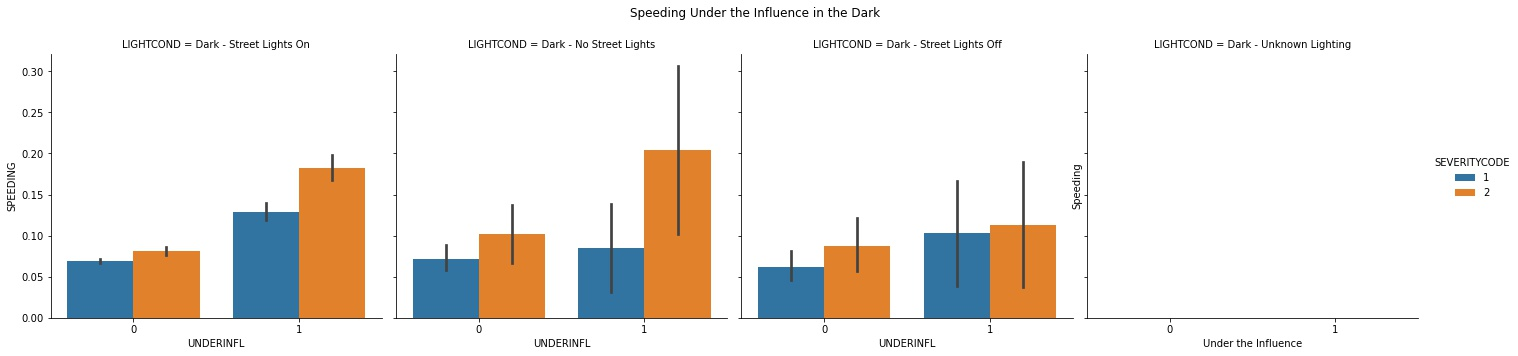
\includegraphics[width=1.1\textwidth]{un_sp_sev_lig.jpg}
	\caption{Speeding under the influence in poor light conditions (Dark lighting)}
	\label{fig5}
\end{figure}


I also explore how the number of vehicles involved in an accident determine if the accident damage property or cause injury. Firstly figure \ref{fig6} distinguishes vehicle count when drivers are either under the influence or not. We note that with odd number of vehicles involved, accidents are more likely to cause injury (blue portion of bar plot) even among sober drivers. On the other hand, when the number of car is even or 2, the accidents is more likely to cause damage to property | most likely the vehicles involved | than causing an injury. Figure \ref{fig7} shows the same result for sober drivers when we consider car speed.\\

\begin{figure}[H]
	\centering
	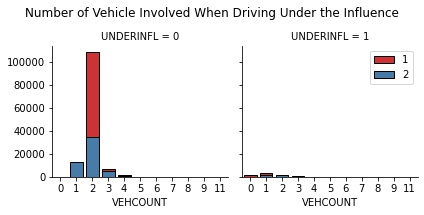
\includegraphics[width=1.0\textwidth]{un_sev_hist.jpg}
	\caption{Vehicle counts and accidents severity when drivers are under the influence.}
	\label{fig6}
\end{figure}

\begin{figure}[H]
	\centering
	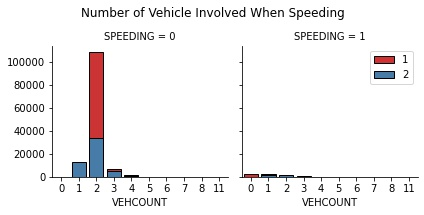
\includegraphics[width=1.0\textwidth]{sp_sev_hist.jpg}
	\caption{Vehicle counts and accidents severity when drivers speed.}
	\label{fig7}
\end{figure}

\subsection{Data Transformation}
This section discusses the transformation of categorical features in the dataset. I use three methods of categorical variable encoding that suits the feature based on the number of levels in the variable. The methods are :-

\begin{enumerate}
  \item Dummy Label Encoding : This method assigns a value of 1 to N depending on the number of categories N. I use the dummy label encoding to transform the 'under the influence' variable to take values of 1 if the driver was under the influence of psychoactive substance and 0 otherwise. Also, I replace 'HIT A PARKED CAR' from ['N', 'Y'] to [0, 1].

  \item One-hot-encoding : This methods create a dummy variable that takes a value of 0 and 1 for every category in a feature. The disadvantage of this method is that it can create so many new binary variables when the feature have multiple categories. The multiple binary variables might only explain a small proportion of total variation in the outcome. To reduce this problem in the machine learning model, I use this method for features with a maximum of three categories. The feature ADDR with categories Block, Intersection and alley was transformed and 'alley' class was dropped to prevent overfitting. Also, I use it to code if the driver was speeding or not.

  \item Frequency Encoding : Another method for coding categorical variable is assigning the value of the frequency of each category in the dataset according to the category in the feature. I construct frequency variables for collision type recorded in the dataset and weather condition.

  \item Probability Odds Encoding : For road and light conditions, I use the probability odds of these conditions leading to an accident causing injuries. For each category group, I divide the probability of accident causing injury by the probability of accident resulting in damage to property in the same category.

\end{enumerate}


\subsection{Descriptive Statistics}
\begin{table}[!htbp] \centering \scriptsize
  \caption{Descriptive Statistics}
  \label{tab1}
\begin{tabular}{@{\extracolsep{5pt}}lccccc}
\\[-1.8ex]\hline
\hline \\[-1.8ex]
Total & \multicolumn{1}{c}{N} & \multicolumn{1}{c}{Mean} & \multicolumn{1}{c}{St. Dev.} & \multicolumn{1}{c}{Min} & \multicolumn{1}{c}{Max} \\
\hline \\[-1.8ex]
SEVERITYCODE      &  182660.0 &  0.31 &  0.46 &  0.00 &   1.00 \\
PERSONCOUNT       &  182660.0 &  2.48 &  1.37 &  0.00 &  81.00 \\
VEHCOUNT          &  182660.0 &  1.97 &  0.56 &  0.00 &  12.00 \\
UNDERINFL         &  182660.0 &  0.05 &  0.22 &  0.00 &   1.00 \\
ADDR\_Block        &  182660.0 &  0.65 &  0.48 &  0.00 &   1.00 \\
ADDR\_Intersection &  182660.0 &  0.35 &  0.48 &  0.00 &   1.00 \\
COLLISIONFREQ     &  182660.0 &  0.16 &  0.07 &  0.01 &   0.25 \\
JUNCTION\_FREQ     &  182660.0 &  0.34 &  0.14 &  0.00 &   0.46 \\
WEATHER\_FREQ      &  182660.0 &  0.41 &  0.22 &  0.00 &   0.59 \\
ROAD\_ODDS         &  182660.0 &  0.45 &  0.11 &  0.05 &   0.60 \\
LIGHT\_ODDS        &  182660.0 &  0.45 &  0.11 &  0.05 &   0.57 \\
SPEED\_N           &  182660.0 &  0.95 &  0.22 &  0.00 &   1.00 \\
ST\_freq           &  182660.0 &  0.12 &  0.08 &  0.00 &   0.23 \\
HITPARKEDCAR      &  182660.0 &  0.03 &  0.17 &  0.00 &   1.00 \\
\hline \\[-1.8ex]
\end{tabular}

	\raggedright\footnotesize \justify { \textit{Notes-} The table is the summary statistics of some of the features in the SDOT dataset. The target variable of interest is the severity code | coded as 0 for accidents that destroy property and 1 for accidents that causes injuries. Some of the dummy features in the dataset has been tranformed using either a binary or one-hot-code dummy tranformation.}

\end{table}



Table \ref{tab1} presents the summary statistics of the SDOT dataset. The target variable, SEVERITYCODE has a mean value of 0.31. This suggests that 31\% of the accidents recorded in the data are accidents that resulted in injuries. The mean number of vehicle involved in accidents in Seattle is 2. 5\% of the accidents came from drivers under the influence of psychoactive substances and only 3\% of the accidents resulted from hitting a parked car.

\subsection{Machine Learning Algorithm}
To predict the severity of accidents, I employ 3 supervised machine learning algorithm. The models are supervised because the target labels are known as either accident causing property damage and accidents causing injury as 0 and 1 respectively. As opposed to regression analysis used in cases of continuous target, I use these classification models that are appropriate for discrete target labels. The three machine learning algorithms are K-Nearest Neighbour (KNN), Decision Tree classification and Logistic model.

\begin{enumerate}
  \item K-Nearest Neighbour (KNN) : The KNN works by assigning a new accident observation to either lead to damage properties or cause injury based on a voting algorithm. I will determine the optimal number of K candidates to vote and assigns the new observation on the target value with the highest occurrence. The closest K are calculated using the euclidean distance. To get the optimal K, I will run the KNN model on multiple Ks and plot the accuracy score and pick the K that produces the highest accuracy in the model.

  \item Decision Tree : Decision trees assign observation to a target class by creating a tree using the observed features as branches and leaf. The algorithm splits the data into groups using the features in the data set from the most important feature till it gets to the purest possible node where all observations are as similar as possible.

  \item Logistic Classifier : The logistic model is similar to regression models but specifically for discrete target values as is the case with accident severity. In this case, the expected values of the linear feature is transformed using a sigmoid linkage function that maps the predicted value of the model between 0 and 1.
\end{enumerate}

The project will test and compare the accuracy of the three classification models. The best performing model will be selected as the best predictor of accident severity.

\section{Results Section}
Previous sections of the research explored the datset. From the exploration, we suspect that the best set of features for predicting accident severity should involve the interaction of the variables in the feature set. For this reason, for the three machine learning model, I will specify two models | one with linear feature and another as polynomial of degree=3 | which interacts in all possible ways every variable in the set.

\subsection{Selecting the Optimal Number of K in the KNN}
One of the main challenges for the K-nearest neighbour is knowing the number of Ks for which the classification voting takes place. Figure \ref{fig8} and \ref{fig9} shows the number of K that produces the best accuracy with a linear and polynomial feature respectively. The graph shows that for both KNN models, K=24 provides the most accurate model in the test set.

\begin{figure}[H]
	\centering
	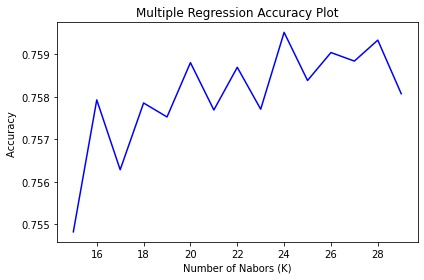
\includegraphics[width=0.6\textwidth]{KNN.jpg}
	\caption{Selecting the optimal K for linear feature KNN classifier}
	\label{fig8}
\end{figure}

\begin{figure}[H]
	\centering
	\includegraphics[width=0.6\textwidth]{KNN_poly.jpg}
	\caption{Selecting the optimal K for polynomial feature KNN classifier}
	\label{fig9}
\end{figure}

\subsection{Model Evaluation}
\begin{table}[!htbp] \centering \scriptsize
  \caption{Accuracy Test Report}
  \label{tab2}
\begin{tabular}{@{\extracolsep{3pt}}lccc}
\\[-1.8ex]\hline
\hline \\[-1.8ex]
Model & \multicolumn{1}{c}{Jaccard} & \multicolumn{1}{c}{F-1 Score} & \multicolumn{1}{c}{Log-Loss}\\
\hline \\[-1.8ex]
 \textbf{KNN \textit{(Linear)}} & \textbf{0.76} & \textbf{0.75} & \textbf{NA} \\
      \textit{(Polynomial)} & 0.74  & 0.68 & NA \\
& & & \\
Decision Tree \textit{(Linear)} & 0.76   &   0.74  & NA      \\
     \textit{(Polynomial)}  & 0.76     & 0.74     & NA     \\
& & & \\
 Logistic  textit{(Linear)} & 0.72     & 0.68     & 0.55    \\
     \textit{(Polynomial)} & 0.75     & 0.71     & 0.50    \\
\hline \\[-1.8ex]
\end{tabular}

	\raggedright\footnotesize \justify { \textit{Notes-} The table presents the Jaccard accuracy, F1-score and log-loss for the three machine learning models used in predicting accident severity. For each model, the top row provides test for linear estimation while the bottom rows are the scores for the models with polynomial features. The best model by Jaccard and F1-score is the KNN with linear features in bold. }

\end{table}



Table \ref{tab2} presents the accuracy test result for the machine learning models employed in the research. We note that across all model types, there was no improvement in using polynomial features that capture interaction effect. This is contrary to our expectation from the exploratory data analysis. We also note that all the machine learning model performance were similar with KNN being the best by a margin. The preferred model for predicting the severity of accident and distinguishing between accidents that damage properties and accidents that result in injury is a KNN with linear features and K value of 24. It is worth stating that given how narrow the difference between the two state of accidents are and the absence of some important risk factor the WHO lists as a common cause of accidents, the overall performance of the models were excellent.

\section{Discussion}
The research provides some insights into the predictors of the severity of car accidents. The data exploration shows that most accidents in Seattle occur in clear weather conditions. Majority of the accidents occurred at night in the dark and the absence of street lights. The accident causing effect of street light is even more prominent when drivers are speeding and under the influence of psychoactive substances. Drivers speeding under the influence of drugs in a dark street contributes substantially to the occurrence of accidents that results in injury.\\

The research also created a model that predicts car accidents severity using the available features collected from the SDOT dataset. The machine learning model that best predicts accident severity is the K-Nearest Neighbour with K=20 and linear features which excludes interactive effects.

\subsection{Policy Recommendation}
From the discussion and the results I give the following recommendations to the government. First, the need to provide street lights in prominent roads seems essential to reduce the incident of vehicular accidents in general. Also the government needs to educate the public on the dangers of speeding and using psychoactive substances while driving. An increase in fines and the number of law enforcement officers checking driver's state of consciousness while driving will decrease these behaviour on the streets of Seattle.

\section{Conclusion}
This project uses machine learning algorithms to predict the severity of car accident. More specifically, I distinguish between accidents that destroy properties and accidents that lead to injury. Some of the features of interests are weather condition, driving under the influence, the type of address location (block, intersection or alley), collision type (angle, sideways, rear ended etc.), location of the accidents, the type of junction, road condition, the light condition, speeding, the number of people and the number of vehicle involved in the accident. I conduct an exploratory data analysis to determine the important features that can distinguish between accident severity types. Importantly, I find that speeding under the influence of psychoactive substances in dark road conditions contributed the most to accidents that result in injury. After the EDA, I specify three machine learning models | K-nearest neighbour, Decision tree and Logistic model. The KNN with linear features and k=20 performed best among other specifications in predicting accident severity in Seattle.

\newpage
\section*{References}
World Health Organization (WHO), 2020. Road Traffic Injuries. [online] Who.int. Available at: <https://www.who.int/news-room/fact-sheets/detail/road-traffic-injuries> [Accessed 5 October 2020].\\

Center for Disease Control, (., 2020. CDC - Motor Vehicle Injury - Topics - Did You Know - STLT Gateway. [online] Cdc.gov. Available at: \newline
<https://www.cdc.gov/publichealthgateway/didyouknow/topic/vehicle.html> [Accessed 5 October 2020].\\

WSDOT, 2020. 2019 Washington State Car Accident Statistics & Reports. [online] Davis Law Group, P.S. Available at: <https://www.injurytriallawyer.com/library/car-accident-statistics-seattle-washington-state.cfm> [Accessed 5 October 2020].

\end{document}
